\documentclass[a4paper,man,natbib]{apa6}

\usepackage[english]{babel}
\usepackage[utf8x]{inputenc}
\usepackage{amsmath}
\usepackage{graphicx}
\usepackage[colorinlistoftodos]{todonotes}
\usepackage{listings}
\usepackage{color}

\definecolor{dkgreen}{rgb}{0,0.6,0}
\definecolor{gray}{rgb}{0.5,0.5,0.5}
\definecolor{mauve}{rgb}{0.58,0,0.82}

\lstset{frame=tb,
	language=C++,
	aboveskip=3mm,
	belowskip=3mm,
	showstringspaces=false,
	columns=flexible,
	basicstyle={\small\ttfamily},
	numbers=none,
	numberstyle=\tiny\color{gray},
	keywordstyle=\color{blue},
	commentstyle=\color{dkgreen},
	stringstyle=\color{mauve},
	breaklines=true,
	breakatwhitespace=true,
	tabsize=3
}



\title{Your APA6-Style Manuscript}
\shorttitle{Your APA6-Style Manuscript}
\author{Moyuan Li}
\affiliation{Miami Oxford}

\abstract{Your abstract here.}

\begin{document}
\maketitle

\section{Introduction}
Travelling salesman problem: Given a set of cities and distance between every pair of cities, the problem is to find the shortest possible route that visits every city exactly once and returns to the starting point. This problem is a famous NP hard problem, which means there is no polynomial time know the solution for the problem. However, when the number of city is very small, we can easily figure out the answer. For example, consider the given graph. There are 4 cities, which is 1,2,3,4. We can quickly figure out that the shortest route would be 1+2+3+4=10. However, if we search deep for how we get this out. The answer is that, we generate all the possible route, which is 1*2*3=6 possible ways. What’s more when we are doing this we set 1 as the starting and ending point automatically. Theoretically, the idea is right. Calculate all the possible route and find out the minimum. Although the idea is simple, in real world, there would be much more cities involved. As the number of city goes up, the possible routes would increase like crazy. It will take too much time to calculate it, even we use computer programming. In this case, researchers find some other way to solve this problem, even the answer may not be exactly the right one, it is still very close. 
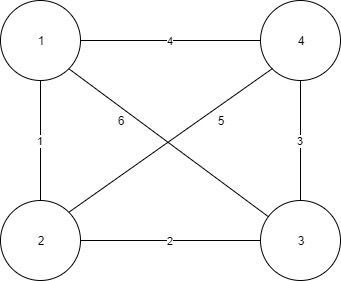
\includegraphics[width=0.5\linewidth]{/home/teddy/cse464/TSP-problem-research/1.png}

\section{Naive/BF implementation}
There are a lot of solutions for the traveling salesman problem. Naïve/BF is the simplest one. The idea about naïve solution is easy to understand. Consider all the possible routes and compare with other and find the lowest cost. The algorithm of naïve/BF implementation is:
\newline1. Consider a city as the starting and ending point.
\newline2. Generate all (n-1) permutations of cities, which means generate all the possible routes.
\newline3. Calculate cost of every permutation and keep track of min cost route.
\newline4. Return the minimum cost route. 
\newline 
The code below is the pseudocode and flowchart for the BF implementation.
\begin{lstlisting}
void brute_force_solver(const Tsp_map& cities) {
Tour tour(cities.get_default_tour());

double best_score = cities.score(tour);
Tour best_tour(tour);
cout << tour << "  score = " << best_score << endl;
while (next_permutation(tour.begin() + 1, tour.end())) {
double s = cities.score(tour);
if (s < best_score) {
best_score = s;
best_tour = tour;
}

cout << tour << "  score = " << s << endl;
} // while
 
cout << "best tour: " << best_tour
<< "\nscore = " << best_score << endl;
\end{lstlisting}
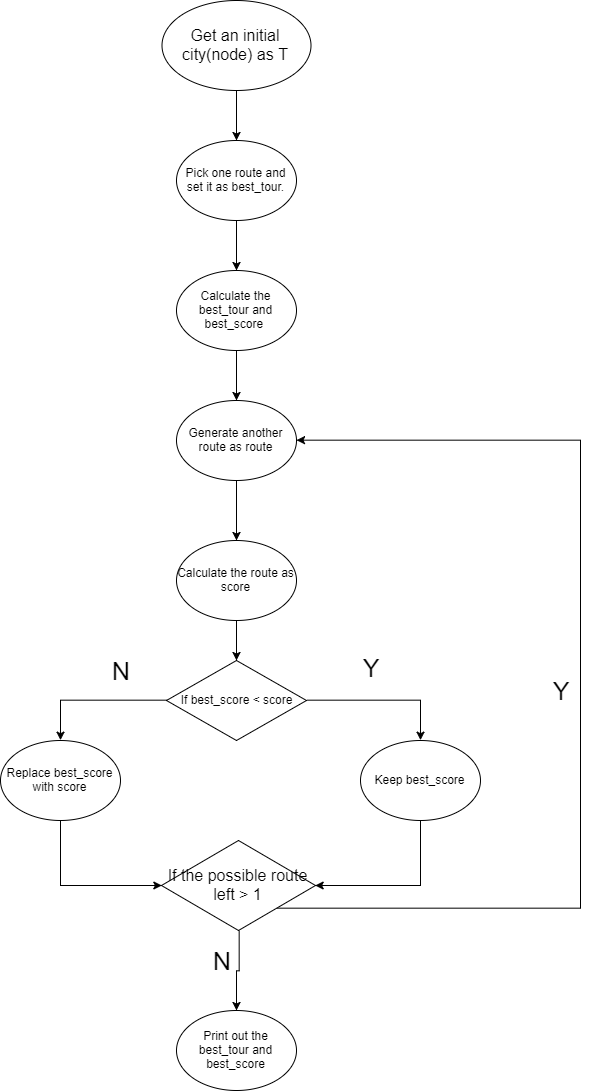
\includegraphics[width=0.5\linewidth]{/home/teddy/cse464/TSP-problem-research/2.png}
Based on the flowchart and pseudocode, we can generate those advantages about the naïve/BF implementation:
\newline1. Naïve/BF implementation will find the most correct route if we have enough time to run this program. (The idea about most correct route I will declare it later in the paper)
\newline2. Simple algorithm, and easy coding.
\newline 
However, we can generate some disadvantages as well.
\newline1. It is not efficient. 
\newline2. It takes too much time to run the program, no one in the real world would ever take so much time to calculate this. Not good for real problem.

\section{Genetic Algorithm}
Since the naive solution is not good enough, researchers need to create some new algorithm to solve the problem. one of those algorithms is called genetic algorithm. It is a meta-heuristic inspired by the nature world, which is the process of natural selection. Implement this genetic algorithm into TSP, it will performance much more better than the naive solution. The idea about genetic algorithm is different than the naive solution. First, we also need to consider a city as starting and ending point, and then generate one route from starting point to ending point. Second, it is the part that different from naive solution. As the algorithm named, we will do the a magic part, which is called crossover and mutation. With this step, we will crossover and mutate our parameter in the TSP problem which will lead to some new routes. Third, find the lowest cost route, and repeat the second step. In order to understand more, we can think the genetic algorithm in this way, you find a route, and then you change some way in the middle of your previous routes. In this case, you will get some different cost of the routes. However, it must have one route is the closest to the correct answer. Thus, we repeat this steps over and over again untill the lowest cost route stop changing. 

\end{document}